% Бүлэг 2

\book{Бизнес эрхлэгчдийн сурталчилгааны нэгдсэн вебийн судалгаа} % Бүлгийн нэр
\label{Chapter2} % Энэ бүлэг рүү ишлэл хийх бол \ref{Chapter1} командыг ашигла 

\section{Системийн үйл ажиллагааны тухай дэлгэрэнгүй }
Энэхүү систем нь реклам зар сурталчилгааг явуулах шаардлагатай үйлдвэрлэл, үйл ажиллагаагаа явуулдаг хувь хүн болоод албан байгуулага, худалдааны гэх мэт бүхий л газрууд өөрт тохируулан ашиглах боломжтой. Реклам зар сурталчилгаа хийхээс гадна хүмүүсийн санал бодлыг хүлээн авах, хариу өгөх зөвлөх зэрэг үйл ажиллагаа байхаас гадна арга хэмжээ, урамшуулалын мэдээллийг хүмүүст хүргэх боломжтой юм.

\section{Системийг ашиглах хэрэглэгчид}
Реклам зар сурталчилгааг нийтэд хүргэх шаардлагатай нийгмийн бүхий л аж ахуйн нэгжүүдэд хэрэглэгдэх боломжтой юм.
Жишээ нь: 
\begin{itemize}
\item Хувиараа бизнес эрхлэгчид
\item Бараа бүтээгдэхүүн үйлдвэрлэгчид
\item Худалдаа наймаачид	
\item Үйл ажиллагаа явуулдаг албан байгуулгууд
\item Хувийн байгуулагууд
\item олон нийтийн байгуулагууд
\item Хувь хүн
\end{itemize}
\section{Функционал шаардлага}
 Энэхүү веб нь хэрэглэгч, админ,зочин гэсэн 3-н оролцогчтой.
Хэрэглэгч нь: Өөрийн үйлдэрлэлийн чиглэлээр хуудас үүсгэн сурталчилах, бусдад түгээх боломжтой.
Админ: Бүх хуудсыг хянах, бүртгэлтэй хэрэглэгч болон вебийн ерөнхий мэдээллийг удирдах.
Зочин:Хуудаснуудын мэдээллийг харах,сэтгэгдэл бичих,үнэлгээ өгөх ба шаардлагатай тохиолдолд бүргүүлэх боломжтой.
Хэрэглэгчийн функциональ шаардлага:
\begin{enumerate}
	\item Өөрийн үйлдвэрлэлийн чиглэлээр вебд хуудас үүсгэх
	\item Хуудсандаа бараа, бүтээгдэхүүний танилцуулага удирдах
	\begin{enumerate}
		\item[2.1] Танилцуулага нэмэх
		\item[2.2] Танилцуулага хасах
		\item[2.3] Өөрчлөх
	\end{enumerate}
	\item Зочидын сэтгэгдэлд хариу бичих
	\item Арга хэмжээ зарлах
\end{enumerate}
Админы функциональ шаардлага:
\begin{enumerate}
	\item Тайлан гаргах
	\begin{enumerate}
		\item[1.1] Вебд хандсан зочидын тайлан
		\item[1.2] Дэлгүүрийн тайлан
	\end{enumerate}
	\item Вебийн бүх хуудсийг удирдах
	\begin{enumerate}
		\item[2.1] Хуудас устгах
		\item[2.2] Хуудсанд сануулга өгөх
	\end{enumerate}
	\item Вебийн ерөнхий реклам зар сурталчилгааг удирдах
	\begin{enumerate}
		\item[3.1] Реклам зар сурталчилгааг устгах
		\item[3.2] Реклам зар сурталчилгааг нэмэх
		\item[3.3] Реклам зар сурталчилгааг өөрчлөх
	\end{enumerate}
\end{enumerate}
Зочины функциональ шаардлага
\begin{enumerate}
	\item Реклам зар сурталчилгаа харах
	\item Реклам зар сурталчилгаанд сэтгэгдэл үлдээх
	\begin{enumerate}
		\item[2.1] Вебд бүртгүүлэх
	\end{enumerate}	
	
	\item Реклам зар сурталгаанд үнэлгээ өгөх
	\begin{enumerate}
		\item[3.1] Вебд бүртгүүлэх
	\end{enumerate}	
	
	\item Арга хэмжээнд санал өгөх
	\item Вебээс хайлт хийх
	\begin{enumerate}
		\item[5.1] Хуудас хайх
		\item[5.2] Арга хэмжээ хайх
	\end{enumerate}
\end{enumerate}
\section{Функционал бус шаардлага}
\begin{enumerate}
	\item Өгөгдлийн сан ачааллах хугацаа нь хурдан шуурхай байх. Бүх өгөгдлүүд өгөгдлийн санд хадгалагдсан байх болно
	\item Вебд 1000-с 10000-хүн нэгэн зэрэг хандаж үйл ажиллагаа явуулах учир серверийн хүчин өндөр байх
	\item Архитектурын хувьд windows орчинд хөгжүүлэгдэнэ.Вебийн хөгжүүлэлт нь CodeIgniter framework – той хамтран ажиллаж боломжтой хэлүүд дээр хийгдэнэ.
	\item Кодчилолын хувьд CodeIgniter framework –ийн стандартын дагуу хийгдэнэ.
\end{enumerate}
\section{Юзкейс диаграм}
\begin{figure}[htbp]
	\centering
	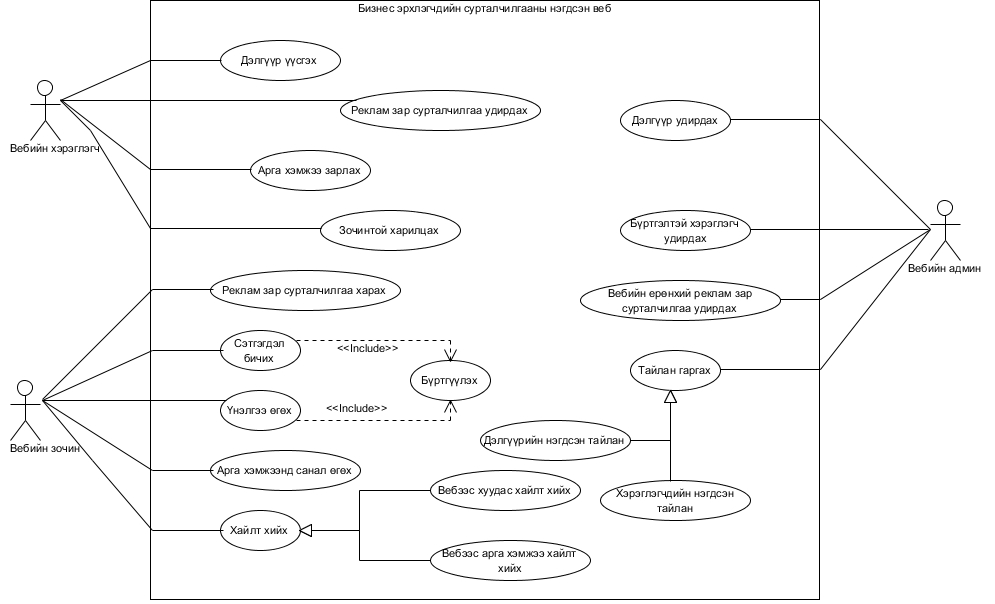
\includegraphics[scale=0.4]{Diagrams/UseCase}
	\caption[Юзкейс диаграм]{Юзкейс диаграм}
	\label{fit:UseCase}
\end{figure}
\section{Юзкейс диаграмын тодорхойлолт}

\begin{center}
	\begin{table}[!htbp]
		\caption{}
		\begin{tabular}{|p{4cm}|p{11cm}|}
		\hline
			Нэр: & Дэлгүүр үүсгэх \\
		\hline
			ID: & 1 \\
		\hline
			Товч тайлбар: & Хэрэглэгч нь веб серверд шинээр бүртгэл үүсгэнэ. \\
		\hline
			Триггер: & Хэрэглэгч нь бүртгүүлэх шаардлагатай болсон. \\
		\hline
			Үндсэн оролцогч: & Хэрэглэгч \\
		\hline
			Хоёрдогч оролцогч: & Байхгүй  \\
		\hline
			Өмнөх нөхцөл: &  Веб сервер ажиллагаатай байх\\
		\hline
			Ажлын урсгал: & \begin{enumerate}
						 	\item Суралцагч нь бүртгүүлэхийг сонгосноор энэ юз кейс эхлэнэ. 
						 	\item Веб сервер нь суралцагчид бүртгүүлэх цонхыг харуулна. 
						 	\item Хэрэглэгч нь өөрийн мэдээллийг (өөрийн нэр, имэйл хаяг, нууц үгээ) оруулна. 
						 	\item Веб сервер нь хэрэглэгчийн оруулсан мэдээллийг шалгана. 
						 	\item IF (“мэдээлэл үнэн зөв бол”)
							 	\begin{enumerate}
							 		\item[5.1] Веб сервер хэрэглэгчийн оруулсан мэдээллийг (өөрийн нэр, имэйл хаяг, нууц үгээ) баазад хадгална.
							 		\item[5.2] Веб сервер хэрэглэгчийг амжилттай бүртгүүлсэнийг нь харуулна. 
							 	\end{enumerate}
						 	\item ELSE
							 	\begin{enumerate}
							 		\item[6.1] Веб сервер нь хэрэглэгчийн оруулсан мэдээлэл бүрийг шалгана.  
							 		\item[6.2] Веб сервер нь алдаатай оруулсан мэдээллийг тодруулж харуулна. 
							 		\item[6.3] Веб сервер нь мэдээллийг дахин оруулахыг асууна. 
							 	\end{enumerate}
						  \end{enumerate}
\\					  \hline
				Дараах нөхцөл: &
				 \begin{enumerate}
									\item Хэрэглэгч веб серверд бүртгэлтэй болсон байна. 
									\item Хэрэглэгчийн мэдээлэл баазад хадгалагдсан байна. 
				\end{enumerate}	   
\\				   \hline
				Альтернатив урсгал: &  \begin{enumerate}
									\item Хэрэглэгч бүртгэлийг цуцалсан.
									\item Веб сервер дээр алдаа гарсан. 
										\end{enumerate}
				\\	\hline
		\end{tabular}
	\end{table}
\end{center}


\begin{center}
	\begin{table}[!htbp]
		\caption{}
		\begin{tabular}{|p{4cm}|p{11cm}|}
			\hline
			Нэр: & Реклам зар сурталчилгаа удирдах \\
			\hline
			ID: & 2 \\
			\hline
			Товч тайлбар: & Хэрэглэгч веб серверд шинээр реклам зар сурталчилгаа нэмнэ.  \\
			\hline
			Триггер: & Хэрэглэгч реклам зар сурталчилгаа нэмэхийг хүссэн. \\
			\hline
			Үндсэн оролцогч: & Хэрэглэгч \\
			\hline
			Хоёрдогч оролцогч: & Веб  \\
			\hline
			Өмнөх нөхцөл: &  \begin{enumerate}
								\item Хэрэглэгч өөрийн эрхээрээ нэвтэрсэн байх.
								\item Веб сервер ажиллагаатай байх.
							\end{enumerate}
\\			\hline
			Ажлын урсгал: & \begin{enumerate}
								\item Хэрэглэгч реклам зар сурталчилгаа нэмэхийг сонгосноор энэ юз кейс эхлэнэ.
								\item Веб нь реклам зар сурталчилгаа нэмэх хуудсыг хэрэглэгчид харуулна.
								\item Хэрэглэгч реклам зар сурталчилгааныхаа замыг зааж өгнө.
								\item Веб тухайн реклам зар сурталчилгаа мөн эсэхийг шалгана.
								\item IF (реклам зар сурталчилгаа байгаа бол)
									\begin{enumerate}
										\item[5.1] Веб тухайн реклам зар сурталчилгааг баазруу ачаална.
										\item[5.2] IF (амжилттай ачаалагдсан бол)
											\begin{enumerate}
												\item[5.2.1] Амжилттай ачаалагдсан мэдээллийг хэрэглэгчид харуулна.
											\end{enumerate}
										\item[5.3] Else
											\begin{enumerate}
												\item[5.3.1] Веб ачаалах үеийн алдааг хэрэглэгчид харуулна.
											\end{enumerate}
										\item[5.4] Веб зөв зам дахин оруулахыг асууна.
								\end{enumerate}
							\end{enumerate}
\\						\hline
			Дараах нөхцөл: &  Вебд реклам зар сурталчилгаа байршисан байна. \\
			\hline
			Альтернатив урсгал: &  Вебийн өгөгдлийн сангын багтаамж дүүрсэн. \\
			\hline
		\end{tabular}
	\end{table}
\end{center}

\begin{center}
	\begin{table}[!htbp]
		\caption{}
		\begin{tabular}{|p{4cm}|p{11cm}|}
			\hline
			Нэр: & Арга хэмжээ зарлах \\
			\hline
			ID: & 3 \\
			\hline
			Товч тайлбар: & Хэрэглэгч өөрийн хуудсаар дамжуулан удахгүй болох арга хэмжээг зарлана.  \\
			\hline
			Триггер: & Хэрэглэгч арга хэмжээ зарлахыг хүссэн. \\
			\hline
			Үндсэн оролцогч: & Хэрэглэгч \\
			\hline
			Хоёрдогч оролцогч: & Байхгүй  \\
			\hline
			Өмнөх нөхцөл: &  \begin{enumerate}
				\item Вебд  өөрийн хуудсаа нээсэн байх.
				\item Веб хэвийн ажиллагаатай байх.
			\end{enumerate}
			\\			\hline
			Ажлын урсгал: & \begin{enumerate}
								\item Хэрэглэгч арга хэмжээ зарлах хэсгийг сонгосоноор энэхүү энэ юзкейс эхэлнэ.
								\item Веб арга хэмжээний тухай бөглөх хуудсыг харуулна
								\item Хэрэглэгч хуудсийг (арга хэмжээ эхлэх, дуусах огноо, тайлбар ) бөглөнө.
								\item IF( Мэдээлэл үнэн бөглөсөн бол )
									\begin{enumerate}
										\item[4.1] Веб арга хэмжээ баталгаажуулах хэсгийг харуулна
									\end{enumerate}
								\item ELSE 
									\begin{enumerate}
										\item[5.1] Веб хэрэглэгчийн оруулсан мэдээлэл алдаатайг мэдэгдэнэ.
										\item[5.2] Хэрэглэгч хуудсыг дахин бөглөнө.
									\end{enumerate}
								\item Хэрэглэгч арга хэмжээг баталгаажуулах хэсгийг сонгоно.
								\item Веб арга хэмжээ амжилттай баталгаажсаныг мэдэгдэнэ.
							\end{enumerate}
\\						\hline
			Дараах нөхцөл: & Арга хэмжээ зарлагдсан байна. \\
			\hline
			Альтернатив урсгал: & Хэрэглэгч арга хэмжээг цуцалсан байна. \\
			\hline
		\end{tabular}
	\end{table}
\end{center}


\begin{center}
	\begin{table}[!htbp]
		\caption{}
		\begin{tabular}{|p{4cm}|p{11cm}|}
			\hline
			Нэр: & Зочинтой харилцах \\
			\hline
			ID: & 4 \\
			\hline
			Товч тайлбар: & Хуудасанд үлдээсэн зочины сэтгэгдэлд хариу бичих.  \\
			\hline
			Үндсэн оролцогч: & Хэрэглэгч \\
			\hline
			Хоёрдогч оролцогч: & Зочин  \\
			\hline
			Өмнөх нөхцөл: &  \begin{enumerate}
				\item Өөрийн хуудсанд нэвтэрсэн байх.
				\item Сэтгэгдэл үлдээсэн зочин вебд бүртгэлтэй байх.
			\end{enumerate}
			\\			\hline
			Ажлын урсгал: & \begin{enumerate}
								\item Хэрэглэгч зочины үлдээсэн сэтгэгдэлд хариу бичих хэсгийг сонгосоноор энэ юзкейс эхэлнэ.
								\item Веб хариу бичих талбарыг нээж харуулна.
								\item Хэрэглэгч зочины сэтгэгдэлд хариу бичнэ.
								\item Хэрэглэгч хариу сэтгэгдэлээ илгээнэ.
								\item Веб хариу сэтгэгдэл амжилттай илгээгдсэнийг мэдэгдэнэ.
							\end{enumerate} \\
						\hline
			Дараах нөхцөл: & Хэрэглэгч зочины сэтгэгдэлд хариу бичсэн байна. \\
			\hline
			Альтернатив урсгал: & Хэрэглэгч бичсэн сэтгэгдэлээ устгасан байна. \\
			\hline
		\end{tabular}
	\end{table}
\end{center}

\begin{center}
	\begin{table}[!htbp]
		\caption{}
		\begin{tabular}{|p{4cm}|p{11cm}|}
			\hline
			Нэр: & Реклам зар сурталчилгаа харах  \\
			\hline
			ID: & 5 \\
			\hline
			Товч тайлбар: & Зочин вебийн реклам зар сурталчилгааг харна.  \\
			\hline
			Үндсэн оролцогч: & Зочин \\
			\hline
			Хоёрдогч оролцогч: & Байхгүй  \\
			\hline
			Өмнөх нөхцөл: &  Вебд нэвтэрсэн байх \\
			\hline
			Ажлын урсгал: &  \begin{enumerate}
								\item Зочин вебд реклам зар сурталчилгаа харах зорилготой нэвтэрсэнээр энэ юзкейс эхэлнэ.
								\item Веб реклам зар сурталчилгааны төрлүүдийг харуулна. 
								\item Зочин реклам зар сурталчилгааныхаа төрлөө сонгоно сонгоно.
								\item Веб зочины сонгосон төрлийг харуулна.  
							\end{enumerate}	 \\
						\hline
			Дараах нөхцөл: & Зочин реклам зар сурталчилгаа харсан байна \\
			\hline 
			Альтернатив урсгал: & Байхгүй \\
			\hline
		\end{tabular}
	\end{table}
\end{center}

\begin{center}
	\begin{table}[!htbp]
		\caption{} 
		\begin{tabular}{|p{4cm}|p{11cm}|}
			\hline
			Нэр: & Сэтгэгдэл бичих  \\
			\hline
			ID: & 6 \\
			\hline
			Товч тайлбар: & Зочин хуудсанд сэтгэгдэл үлдээх.  \\
			\hline
			Үндсэн оролцогч: & Зочин \\
			\hline
			Хоёрдогч оролцогч: & Байхгүй  \\
			\hline
			Өмнөх нөхцөл: &  Вебд бүртгэлтэй байх \\
			\hline
			Ажлын урсгал: & \begin{enumerate}
								\item Зочин сэтгэгдэл үлдээх хэсгийг сонгосоноор энэ юзкейс эхэлнэ
								\item Веб зочинд сэтгэгдэл үлдээх хэсгийг харуулна
								\item Зочин хэсгийг сонгоно
								\item IF( Зочин вебд бүртгэлгүй бол )
									\begin{enumerate}
										\item[4.1] Веб бүртгэлийн хуудсийг харуулна
									\end{enumerate}
								\item ELSE
									\begin{enumerate}
										\item[5.1] Зочин сэтгэгдэл үлдээх хэсэгт сэтгэгдэлээ үлдээнэ
									\end{enumerate}
								\item Зочин сэтгэгдэл баталгаажуулах хэсгийг сонгоно
								\item Веб сэтгэгдэл амжилттай үлдээснийг мэдэгдэнэ.
							\end{enumerate} 	
\\				\hline
			Дараах нөхцөл: & Зочин хуудсанд сэтгэгдэл үлдээсэн байна. \\
			\hline
			Альтернатив урсгал: & Зочин сэтгэгдэлээ устгасан байна. \\
			\hline
		\end{tabular}
	\end{table}
\end{center}

\begin{center}
	\begin{table}[!htbp]
		\caption{} 
		\begin{tabular}{|p{4cm}|p{11cm}|}
			\hline
			Нэр: & Хайлт хийх  \\
			\hline
			ID: & 7 \\
			\hline
			Товч тайлбар: & Зочин вебээс өөрийн хүссэн реклам зар сурталчилгааг хайна.  \\
			\hline
			Үндсэн оролцогч: & Зочин \\
			\hline
			Хоёрдогч оролцогч: & Байхгүй  \\
			\hline
			Өмнөх нөхцөл: &  Вебд нэвтэрсэн байх \\
			\hline
			Ажлын урсгал: & \begin{enumerate}
								\item Зочин хайлт хийх хэсгийг сонгосоноор энэхүү юзкейс эхэлнэ
								\item Веб хайлт хийх төрлүүдийг харуулна харуулна
								\item Зочин хайлт хийх төрөлөө сонгоно
								\item Веб зочины сонгосон хайлт хийх хэсгийг харуулна
								\item Зочин хайлтын утгаа оруулна
								\item IF(Хайлтын утга алдаатай бол)
									\begin{enumerate}
										\item[6.1] Веб хайлтын утга алдаатайг зочинд мэдэгдэнэ.
										\item[6.2] Веб зочинд зөв хайлтын жишээ утга харуулна
									\end{enumerate}	
								\item ELSE IF(Таны хайсан утга )
									\begin{enumerate}
										\item[7.1] Веб таны хайсан утга илэрцгүй 
									\end{enumerate}
								\item Зочин хайлтанд илэрсэн утгуудыг харуулна
							\end{enumerate} 	\\
						\hline
			Дараах нөхцөл: & Зочин вебээс хүссэн хайлтаа олсон байна. \\
			\hline
			Альтернатив урсгал: & Зочины хайлт илэрцгүй байна.\\
			\hline
		\end{tabular}
	\end{table}
\end{center}

\begin{center}
\begin{table}[!htbp]
	\caption{}
	\begin{tabular}{|p{4cm}|p{11cm}|}
		\hline
		Нэр: & Арга хэмжээнд санал өгөх  \\
		\hline
		ID: & 8 \\
		\hline
		Товч тайлбар: & Зочин хуудсануудын арга хэмжээнд санал өгөх боломжтой.  \\
		\hline
		Үндсэн оролцогч: & Зочин \\
		\hline
		Хоёрдогч оролцогч: & Байхгүй  \\
		\hline
		Өмнөх нөхцөл: &  Зочин вебд бүртгэлтэй байх. \\
		\hline
		Ажлын урсгал: & \begin{enumerate}
							\item Зочин арга хэмжээнд санал өгөх хэсгийг сонгосоноор энэ юзкейс эхэлнэ.
							\item Веб арга хэмжээнд санал өгөх хэсгийг харуулна
							\item Зочин санал өгөх хэсгийг сонгоно.
							\item IF( Зочин вебд бүртгэлгүй бол )
								\begin{enumerate}
									\item[4.1] Веб бүртгэлийн хуудсийг харуулна
								\end{enumerate}
							\item ELSE
								\begin{enumerate}
									\item[5.1] Зочин арга хэмжээнд санал өгнө
								\end{enumerate}
							\item Зочин санал баталгаажсаны веб мэдэгдэнэ
						\end{enumerate}	\\
		\hline
		Дараах нөхцөл: & Зочин арга хэмжээнд санал өгсөн байна. \\
		\hline
		Альтернатив урсгал: & Зочин саналаа устгасан байна. \\
		\hline
	\end{tabular}
\end{table}
\end{center}

\begin{center}
	\begin{table}[!htbp]
		\caption{}
		\begin{tabular}{|p{4cm}|p{11cm}|}
			\hline
			Нэр: & Бүртгэлтэй хэрэглэгч удирдах  \\
			\hline
			ID: & 9 \\
			\hline
			Товч тайлбар: & Админ бүртгэлтэй зочиныг вебээс хасах.  \\
			\hline
			Үндсэн оролцогч: & Админ \\
			\hline
			Хоёрдогч оролцогч: & Байхгүй  \\
			\hline
			Өмнөх нөхцөл: &  Зочин вебд зүй зохисгүй зүйл хийх. \\
			\hline
			Ажлын урсгал: & \begin{enumerate}
								\item Админ бүртгэлтэй зочидын жагсаалтыг сонгосоноор энэ юзкейс эхэлнэ.
								\item Веб бүртгэлтэй зочидын жагсаалтыг харуулна
								\item Админ зөрчилтэй зочинг сонгоно
								\item Веб зөрчилтэй зочины мэдээллийг харуулна
								\item Админ зөрчилтэй зочинг вебээс хасна
								\item Веб зөрчилтэй зочин амжилттэй вебээс хасагдсаныг мэдэгдэнэ.
							\end{enumerate}	\\
						\hline
			Дараах нөхцөл: & Зөрчилтэй зочин вебээс хасагдсан байна.(Бүртгэлтэй зочидын сангаас хасагдах ) \\
			\hline
			Альтернатив урсгал: & Админ зочинг буцаан сэргээсэн байна. \\
			\hline
		\end{tabular}
	\end{table}
\end{center}

\begin{center}
	\begin{table}[!htbp]
		\caption{}
		\begin{tabular}{|p{4cm}|p{11cm}|}
			\hline
			Нэр: & Сайтын ерөнхий реклам зар сурталчилгааг удирдах  \\
			\hline
			ID: & 10 \\
			\hline
			Товч тайлбар: & Сайтын ерөнхий реклам зар сурталчилгааг нэмэх, хасах, өөрчлөх боломжтой.  \\
			\hline
			Үндсэн оролцогч: & Админ \\
			\hline
			Хоёрдогч оролцогч: & Байхгүй  \\
			\hline
			Өмнөх нөхцөл: &  Админ эрхээр нэвтэрсэн байх. \\
			\hline
			Ажлын урсгал: & \begin{enumerate}
								\item Админ сайтын ерөнхий реклам зар сурталчилгаа удирдах хэсгийг сонгосоноор энэ юзкейс эхэлнэ
								\item Веб реклам зар сурталчилгаа удирдах төрлүүдийг харуулна
								\item Админ реклам зар сурталчилгаа нэмэх хэсгийг сонгоно
								\item Веб нь реклам зар сурталчилгаа нэмэх хуудсыг админд харуулна.
								\item Админ реклам зар сурталчилгааныхаа замыг зааж өгнө.
								\item Веб тухайн реклам зар сурталчилгаа мөн эсэхийг шалгана.
								\item IF (реклам зар сурталчилгаа байгаа бол)
									\begin{enumerate}
										\item[7.1] Веб тухайн реклам зар сурталчилгааг баазруу ачаална.
										\item[7.2] IF (амжилттай ачаалагдсан бол)
											\begin{enumerate}
												\item[7.2.1] Амжилттай ачаалагдсан мэдээллийг админд харуулна. 
											\end{enumerate}
										\item[7.3] Else
											\begin{enumerate}
												\item[7.3.1] Веб ачаалах үеийн алдааг админд харуулна. 
											\end{enumerate}
										\item[7.4] Веб зөв зам дахин оруулахыг асууна.
									\end{enumerate}
								\item Вебийн ерөнхий реклам зар сурталчилгаа амжилттай нэмэгдсэнийг мэдэгдэнэ.
						\end{enumerate}	\\
					\hline
			Дараах нөхцөл: & Вебийн ерөнхий реклам зар сурталчилгаа нэмэгдсэн байна \\
			\hline
			Альтернатив урсгал: & Админ буцааж устгасан байна \\
			\hline
		\end{tabular}
	\end{table}
\end{center}
%-------------------------------------------------------------------------------
\section{Шинжилгээний класс диаграм}

\begin{figure}[!h]
	\centering
	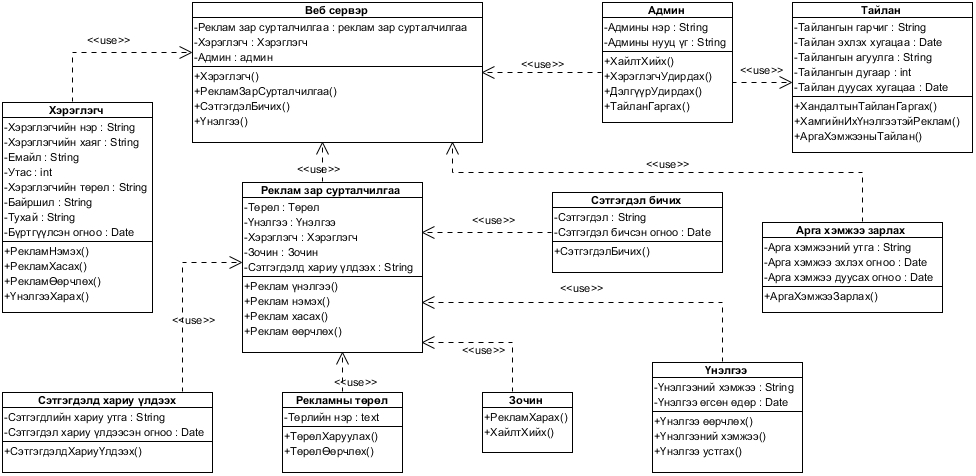
\includegraphics[angle=90,scale=0.7]{Diagrams/SClass}
	\caption[Шинжилгээний класс диаграм]{Шинжилгээний класс диаграм}
	\label{fig:SClass}
\end{figure}

%--------------------------------------------------------------
\section{Шинжилгээний дарааллын диаграм}
\begin{figure}
	\centering
	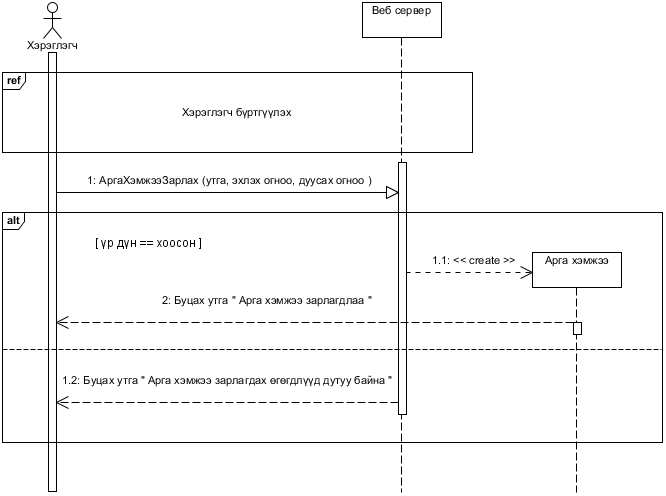
\includegraphics[scale=0.7]{Diagrams/arga_hemjee}
	\caption[Арга хэмжээ зарлах шинжилгээний дарааллын диаграм]{Арга хэмжээ зарлах шинжилгээний дарааллын диаграм}
	\label{text}
\end{figure}

\begin{figure}
	\centering
	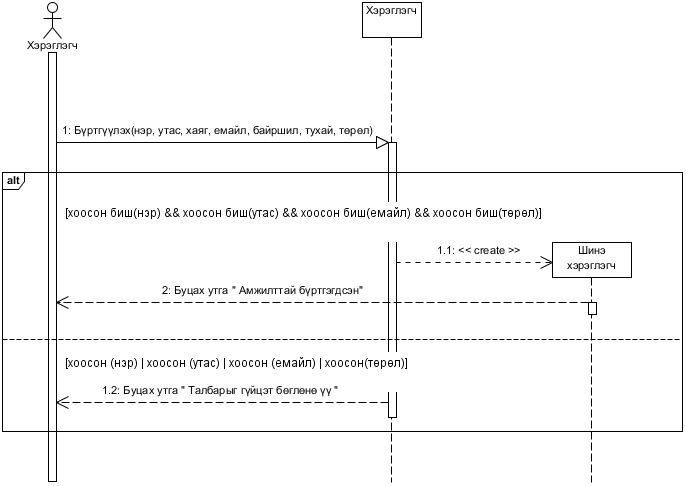
\includegraphics[scale=0.65]{Diagrams/create}
	\caption[Бүртгүүлэх шинжилгээний дарааллын диаграм]{Бүртгүүлэх шинжилгээний дарааллын диаграм}
	\label{text}
\end{figure}

\begin{figure}
	\centering
	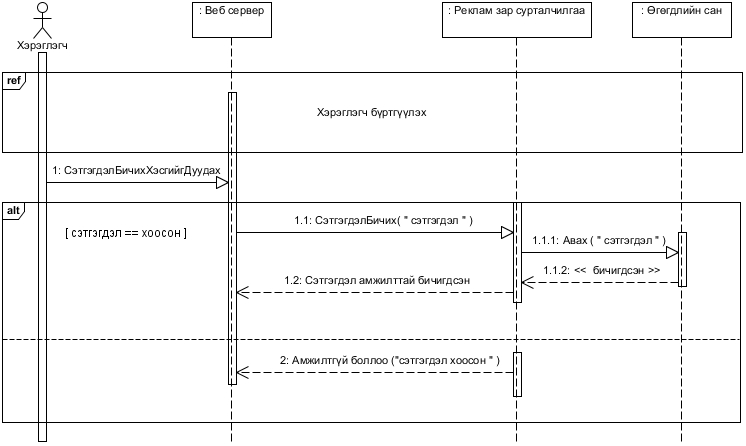
\includegraphics[scale=0.6]{Diagrams/write}
	\caption[Сэтгэгдэл бичих шинжилгээний дарааллын диаграм]{Сэтгэгдэл бичих шинжилгээний дарааллын диаграм}
	\label{text}
\end{figure}

\section{Үйл ажиллагааны диаграм}
\begin{figure}
	\centering
	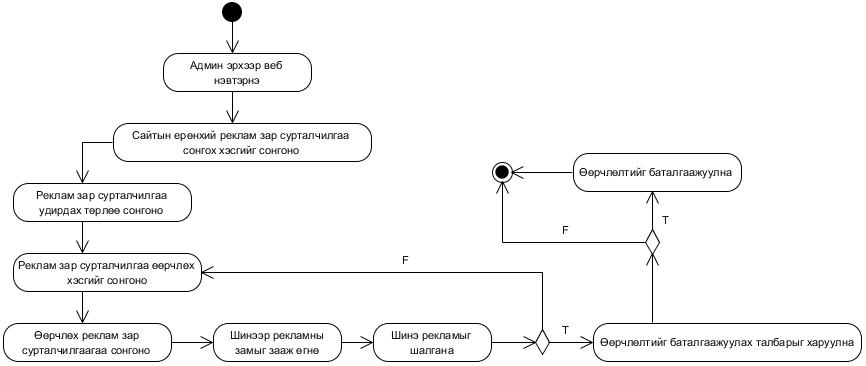
\includegraphics[scale=0.5]{Diagrams/change}
	\caption[Сайтын ерөнхий реклам удирдах үйл ажиллагааны диаграм]{Сайтын ерөнхий реклам удирдах үйл ажиллагааны диаграм}
	\label{text}
\end{figure}
\begin{figure}
	\centering
	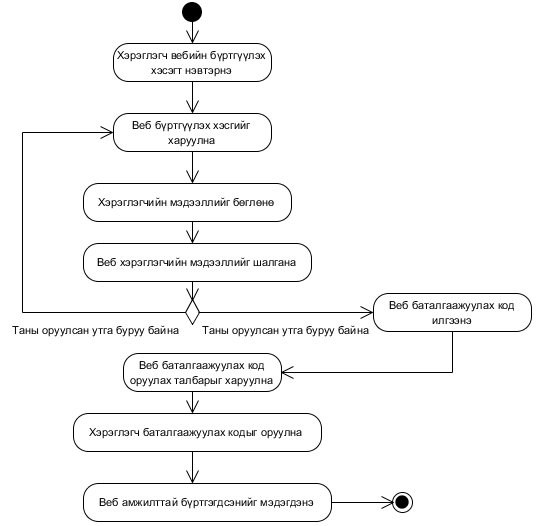
\includegraphics[scale=0.75]{Diagrams/sign_up}
	\caption[Бүртгүүлэх үйл ажиллагааны диаграм]{Бүртгүүлэх үйл ажиллагааны диаграм}
	\label{text}
\end{figure}
\begin{figure}
	\centering
	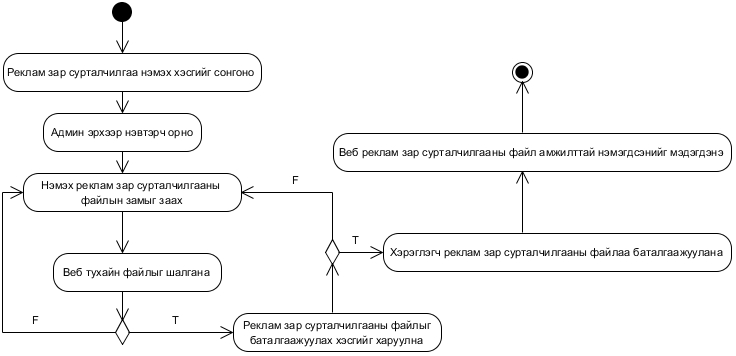
\includegraphics[scale=0.6]{Diagrams/add}
	\caption[Реклам зар сурталчилгаа нэмэх үйл ажиллагааны диаграм]{Реклам зар сурталчилгаа нэмэх үйл ажиллагааны диаграм}
	\label{text}
\end{figure}
\begin{figure}
	\centering
	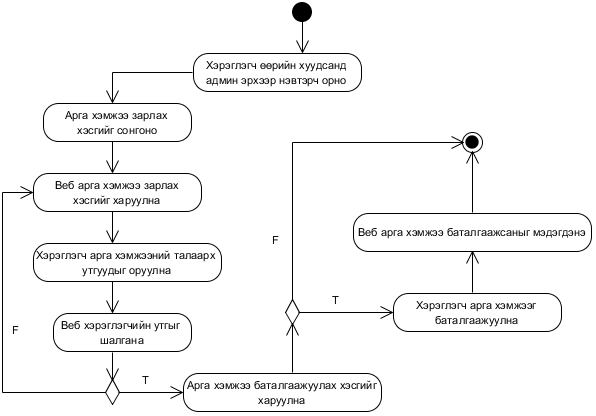
\includegraphics[scale=0.75]{Diagrams/event}
	\caption[Арга хэмжээ зарлах үйл ажиллагааны диаграм]{Арга хэмжээ зарлах үйл ажиллагааны диаграм}
	\label{text}
\end{figure}
\begin{figure}
	\centering
	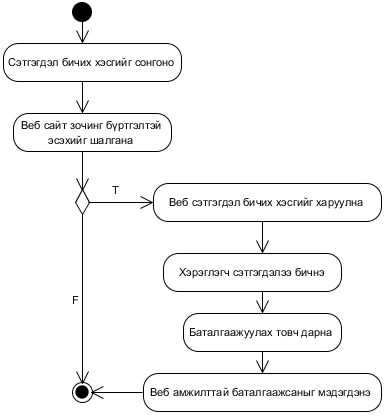
\includegraphics[scale=0.75]{Diagrams/comment}
	\caption[Сэтгэгдэл бичих үйл ажиллагааны диаграм]{Сэтгэгдэл бичих үйл ажиллагааны диаграм}
	\label{text}
\end{figure}w

\begin{figure}
	\centering
	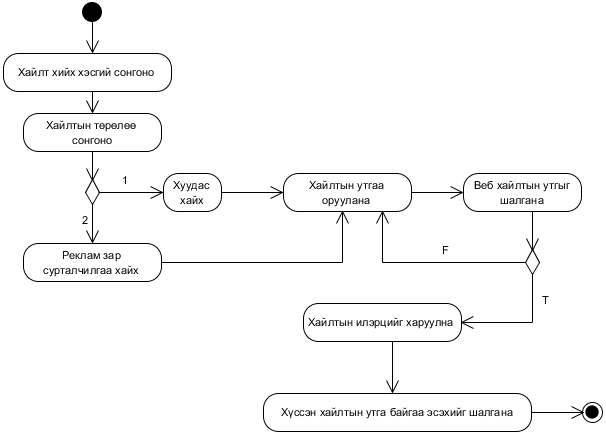
\includegraphics[scale=0.7]{Diagrams/search}
	\caption[Хайлт хийх үйл ажиллагааны диаграм]{Хайлт хийх үйл ажиллагааны диаграм}
	\label{text}
\end{figure}


\section{Бүлгийн дүгнэлт}
Хэрэглэгчийн шаардлагаа тодорхойлж тодорхойлсон шаардлага бүрээ нягтлан хянаж функционал болон фунционал бусаар нь ялгасан. Функционал шаардлага дээрээ үндэслэн юз кейс диаграмаа гаргасан ба бүх  юзкейс бүрт тодорхойлолт гаргасан. Мөн тодорхойлолт бичсэн юзкейс диаграм бүртээ үйл ажиллагааны диаграм зурсан үйл ажиллагааг нь илүү нарийн ойлгомжтой болгож өгч байна.

